\chapter{Spontansprachliche Vorgänge}

Auch wenn Spontansprache durch viel Variabilität charakterisiert ist, so sind viele spontansprachliche Vorgänge dennoch regelhaft. Diese lassen sich als phonologische Prozesse und Regeln beschreiben.

\section{Stichworte zur Vorlesung \em{Phonologische Prozesse und Regeln}}
Neutralisierung, Assimilation, Fortisierung/Lenisierung, Epenthese, Tilgung, Längung, Kürzung, Metathese, Reduplikation $\rightarrow$ {\tt L9\underline{\ }Spontansprache.pdf}

\begin{figure}[htbp]
\begin{center}
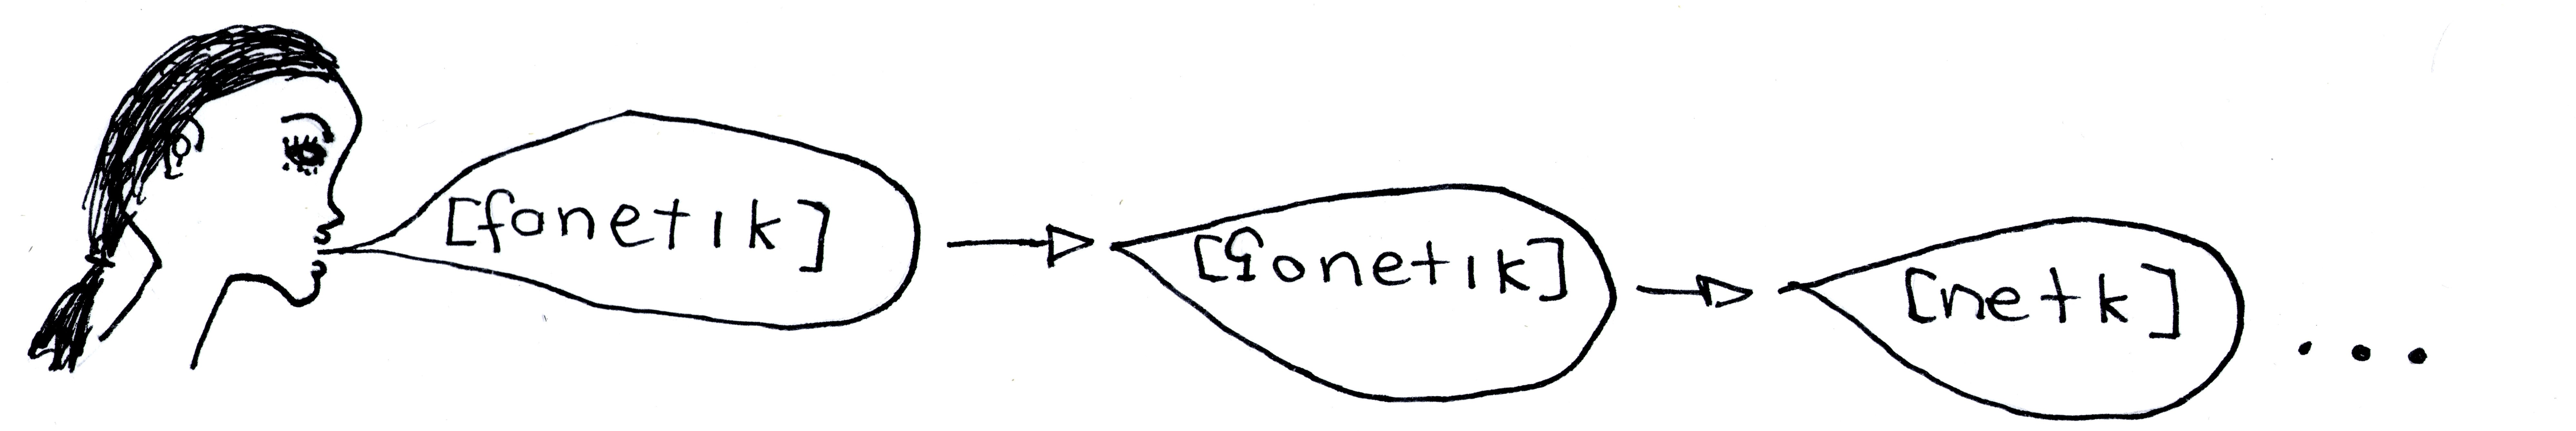
\includegraphics[width=\textwidth]{grafiken/spontansprachliche-vorgaenge/phonologische-prozesse.jpg}
\label{t7}
\end{center}
\end{figure}

\newpage
\section{Übungen}
1.	Identifizieren und erklären Sie die phonologischen Prozesse in den Daten:

\begin{center}
\begin{tabular} {|p{3cm}|p{3cm} |l|l|} \hline
peel [pi:l]&pool [p\super{w}u:l]\\ \hline
tea [ti:]&two [t\super{w}u:]\\ \hline
she [\textesh i:]&shoe [\textesh \super{w}u:]\\ \hline
leek [li:k]&Luke [l\super{w}u:k]\\ \hline
get [get]&got [g\super{w}ot]\\ \hline
\end{tabular}\vspace{1cm}\\
\end{center}

\begin{center}
\begin{tabular} {|p{3cm}|p{3cm} |l|l|} \hline
in-legal&illegal\\ \hline
in-licit&illicit\\ \hline
in-rational&irrational\\ \hline
in-revocable&irrevocable\\ \hline
in-possible&impossible\\ \hline
in-polite&impolite\\ \hline
in-patient&impatient\\ \hline
\end{tabular}
\end{center}
